\subsection{Data Injection On The Grid Processor}
We utilize the $\sigma^{\star}$ to present $-(\sigma+1)$.  
The flow matrix closed-form of \Fig{rt0} is:
\begin{equation}
{
\left[ \begin{array}{ccccccc}
1 & 4 & 8 & 10 & 8 & 4 & 1\\
1 & \sigma^{\star} & 0 & 0 & 0 & 0 & 0\\
1 & -\sigma & \sigma^{\star} & 0 & 0 & 0 & 0\\
1 & -\sigma & -\sigma & -\sigma^{\star} & 0 & 0 & 0\\
1 & -\sigma & -\sigma & -\sigma & \sigma^{\star} & 0 & 0\\
1 & -\sigma & -\sigma & -\sigma & -\sigma & \sigma^{\star} & 0\\
1 & -\sigma & -\sigma & -\sigma & -\sigma & -\sigma & \sigma^{\star}
\end{array} 
\right ]} \times \left[ \begin{array}{c}
\alpha_{0} \\
\alpha_{1} \\
\alpha_{2} \\
\alpha_{3} \\
\alpha_{4}\\
\alpha_{5}\\
\alpha_{6}\\
\end{array} 
\right ] = \left[ \begin{array}{c}
1 \\
0 \\
0 \\
0 \\
0\\
0\\
0
\end{array} 
\right ]
\end{equation}
The fraction curve result is :

\begin{figure}[!ht]
\centering
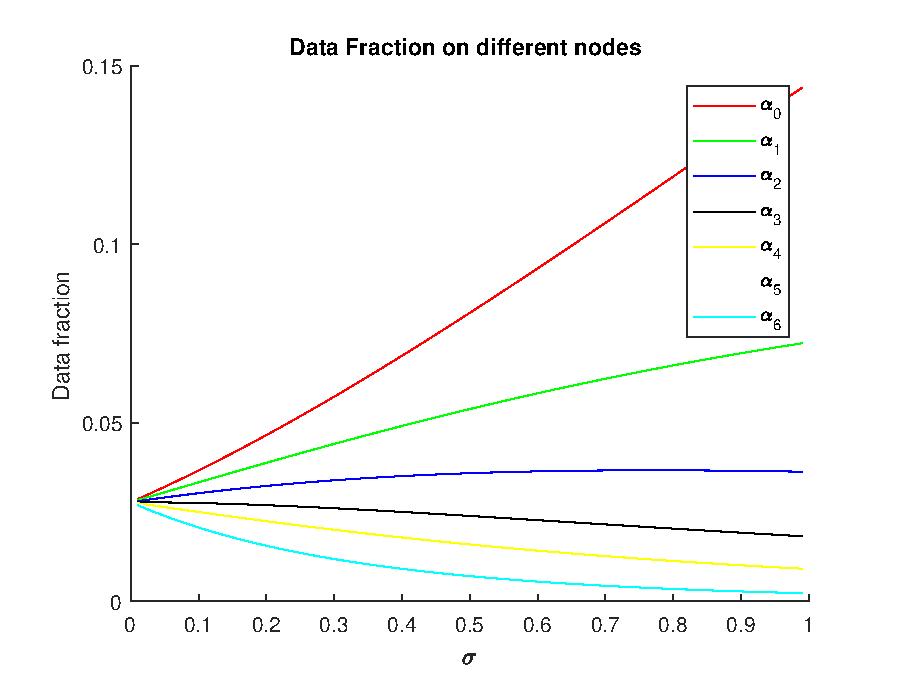
\includegraphics[width=1\columnwidth]{figure/rt_no_fraction.eps}
\caption{The data fraction curve of \Fig{rt0} }
\label{fig:rt_no_fraction}
\end{figure}

From \Fig{rt_no_fraction},  we see that as the value $\sigma$ grows, more and more workload is assigned to the $P_{4, 2}$ and its one hop neighbors.   That is,  as the communication ability decades,  the economical method is to locally process the job. 
\newpage